% !TEX program = xelatex
% 完整编译方法 2: xelatex -> bibtex -> xelatex -> xelatex
% Auriga theme
% https://github.com/anishathalye/auriga

\documentclass[14pt,aspectratio=169]{beamer}
\usepackage{pgfpages}
\usepackage{fancyvrb}
\usepackage{tikz}
\usepackage{pgfplots}
\usepackage{xeCJK}
\setCJKmainfont{FandolSong-Regular}
\setCJKsansfont[
    BoldFont=FandolSong-Bold,
    ItalicFont=FandolKai-Regular
]{FandolSong-Regular}
\setCJKmonofont{FandolFang-Regular.otf}
\newCJKfontfamily\kai[AutoFakeBold=true]{FandolKai-Regular}
\newCJKfontfamily\hei{SimHei}
 % 中文字体设定

\usetheme{auriga}
\usecolortheme{auriga}

% define some colors for a consistent theme across slides
\definecolor{red}{RGB}{181, 23, 0}
\definecolor{blue}{RGB}{0, 118, 186}
\definecolor{gray}{RGB}{146, 146, 146}

\title{标题}

\author{\underline{\bf\kai{张三}} \inst{1} \and {\bf\kai{李四}} \inst{2} \and {\bf\kai{王五}} \inst{3}}

\institute[shortinst]{\inst{1} 北京师范大学 \samelineand \inst{2}
四川联合大学 \samelineand \inst{3} 山东德州大学}

\begin{document}

{
  % rather than use the frame options [noframenumbering,plain], we make the
  % color match, so that the indicated page numbers match PDF page numbers
  \setbeamercolor{page number in head/foot}{fg=background canvas.bg}
  \begin{frame}
    \titlepage
  \end{frame}
}

% !TEX root = *-cn.tex

\begin{frame}{中文字体测试}
    \begin{itemize} % [<+- | alert@+>]
        \item 缺省字体,\textbackslash textbf \textbf{粗体},
            \textbackslash textit \textit{斜体}
        \item \textbackslash alert \alert{字体},
            \textbackslash emph \emph{强调字体}
        \item \textbackslash hei \hei{黑体},
            \textbackslash kai \kai{楷体},
            \textbackslash texttt \texttt{字体},
            \textbackslash textsf \textsf{字体}
        \item \textbackslash bfseries {\bfseries \kai{粗楷体}},
            \textbackslash textbf \textbf{\kai{粗楷体}}
    \end{itemize}
\end{frame}
 % 中文字体测试
\begin{frame}{A slide title}

  \begin{itemize}
    \item A bulleted item
    \item Another item
      \begin{itemize}
        \item With sub-bullets
        \item And another, with some \textbf{bold} text
      \end{itemize}
    \item And another, at the top level, with \textit{italic} text
  \end{itemize}

  \note{
    Here's a note for this slide.
  }

\end{frame}

\begin{frame}{A 50-50 split slide}

  \begin{columns}
    \begin{column}{0.5\linewidth}
      \begin{itemize}
        \item This side has a bullet
        \item And another bullet, with text that wraps if it's long
      \end{itemize}
    \end{column}
    \begin{column}{0.5\linewidth}
      \begin{figure}
        \centering
        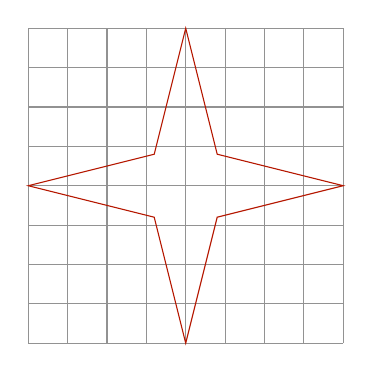
\begin{tikzpicture}[scale=2]
          \draw[step=0.25cm,color=gray] (-1,-1) grid (1,1);
          \draw[color=red] (1,0) -- (0.2,0.2) -- (0,1) -- (-0.2,0.2) -- (-1,0)
          -- (-0.2,-0.2) -- (0,-1) -- (0.2,-0.2) -- cycle;
        \end{tikzpicture}
        \caption{A figure caption}
      \end{figure}
    \end{column}
  \end{columns}

  \note{
    This slide has notes too.
  }

\end{frame}

\begin{frame}{Full-slide figure}

  \begin{figure}
    \centering
    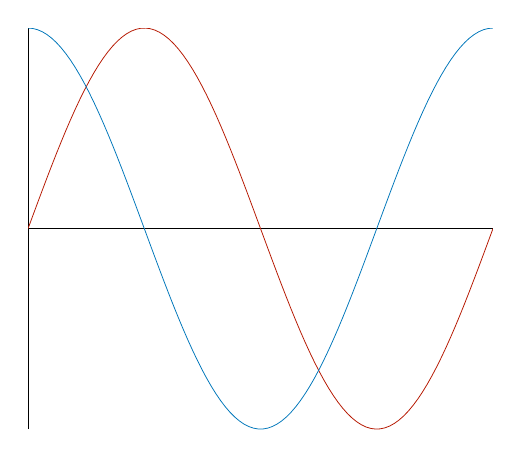
\begin{tikzpicture}[scale=0.7]
      \begin{axis}[
          scale only axis,
          no markers,
          domain=0:2*pi,
          samples=100,
          axis lines=center,
          axis line style={-},
          ticks=none]
        \addplot[red] {sin(deg(x))};
        \addplot[blue] {cos(deg(x))};
      \end{axis}
    \end{tikzpicture}
    \caption{The figure's caption}
  \end{figure}


\end{frame}

\begin{frame}{A slide with centered text}

  \begin{center}
    Some statement that is centered.
  \end{center}

  \vspace{2ex}
  \begin{center}
    \scriptsize (a small note)
  \end{center}

\end{frame}

\begin{frame}[fragile]{A slide with some code}

	\begin{columns}
		\begin{column}{0.5\linewidth}
			\footnotesize
			\begin{Verbatim}[commandchars=\\\{\}]
/* some code */
def foo(x):
  return x**0.5 + 2*x

\color{blue}/* some can be highlighted */
\color{blue}foo(3)
      \end{Verbatim}
    \end{column}
    \begin{column}{0.5\linewidth}
      {\color{red} Some explanatory text, in red, with some \texttt{monospace} text.}
      There might be some math, too:

      $$\sqrt{x} + 2x$$
    \end{column}
  \end{columns}

\end{frame}

\begin{frame}{A slide with some bracketed text}

	\begin{itemize}
		\item Some statement {\color{gray} [Some citation]}
		\item Another statement {\color{gray} [Another citation]}
		\item A final statement {\color{gray} [The last citation]}
	\end{itemize}

	\vspace{3ex}
	\begin{center}
		\scriptsize (a small note)
	\end{center}

\end{frame}


\begin{frame}{A slide with some text and a link}

  \begin{itemize}
    \item This slide has some text along with a link
      \begin{itemize}
        \item \textbf{Some bold text}: followed by an explanation
        \item \textbf{More bold text}: followed by more text
      \end{itemize}
    \item Another bullet, with sub-bullets
      \begin{itemize}
        \item A sub-bullet
        \item Another sub-bullet, with more text
      \end{itemize}
  \end{itemize}

  \vspace{2ex}
  \begin{center}
    \color{blue} \href{https://github.com/anishathalye/auriga}{github.com/anishathalye/auriga}
  \end{center}

\end{frame}


\end{document}
